\documentclass{beamer}
\mode<presentation>
{
\usepackage{dis-template}
}
\usepackage{listings}
\usepackage{hyperref}
\usepackage{textcomp}
\usepackage{soul}
\usepackage{color}
\definecolor{comments}{HTML}{50c878}
\lstset{language=C++,
  basicstyle=\ttfamily,
  keywordstyle=\color{blue}\ttfamily,
  stringstyle=\color{red}\ttfamily,
  commentstyle=\color{comments}\ttfamily,
  breaklines=true
}
\graphicspath{{slides/}} % TODO: eliminate this hack, necessary because scons builds at repository root

%---------------------------------------------------------------------
\titlepageinit{3}{Motor Driver and Servo Control}{4 \& 5 Feb 2015 (Week 3)}
%---------------------------------------------------------------------
\begin{document}
%---------------------------------------------------------------------
\begin{frame}
\titlepage

\setcounter{tocdepth}{1}
\tableofcontents
\end{frame}

% LAB PREPARATION
% Set up function generator to circuit
%   Yellow: function generator out
%   Blue: gate driver out
%   Purple: motor- (signal, to transistor)
%   Green: motor+ (+vsupply)
%   Red (math): voltage across motor, ch4 - ch3
% Get solid and stranded wire, feel the difference

%---------------------------------------------------------------------
\section{Motor Driver Circuits} % [?? mins]
%---------------------------------------------------------------------
\begin{frame}
\centering \huge Motor Driver Circuits
\end{frame}

% TODO: Motor driver topologies refresher
% Shout out advantages and disadvantages of each circuit
% One-transistor
% Half-bridge
% Full H-bridge
% Shout out modes of full H-bridge operation
% Shoot-through and hardware protection
% ... and MOSFETs lighting on fire

\subsection{Motor Driver Topologies}

\begin{frame}
\frametitle{Single-Transistor Recap \small (for your reference)}
\begin{columns}[t]
\column{0.646\textwidth}
\begin{itemize}
  \item This simple driver design gives you on/off control while only needing one transistor
  \item<2-> When the switch is off, no current can flow and the motor freewheels
  \item<3-> When the switch is on, current flows through the motor, causing it to spin
\end{itemize}

\column{0.323\textwidth}
\begin{figure}
  \centering
  \only<1>{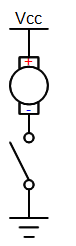
\includegraphics[width=0.33\columnwidth]{images-dis3/driver-single} \\ Single-transistor driver}
  \only<2>{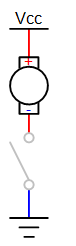
\includegraphics[width=0.33\columnwidth]{images-dis3/driver-single-off} \\ Motor off}
  \only<3>{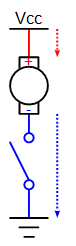
\includegraphics[width=0.33\columnwidth]{images-dis3/driver-single-on} \\ Motor on}
\end{figure}
\end{columns}
\end{frame}

\begin{frame}
\frametitle{Half-Bridge Recap \small (for your reference)}
\begin{columns}[t]
\column{0.646\textwidth}
\begin{itemize}
  \item This driver design gives you drive and braking control using two transistors
  \item<2-> When both switches are off, no current can flow and the motor freewheels
  \item<3-> When the bottom switch is on, current flows through the motor, causing it to spin
  \item<4-> When the top switch is on, the motor's voltage is applied back across itself, applying braking force
  \item<5-> Never turn on both transistors on at once - this shorts the supply across the transistors
  \begin{itemize}
    \item<5-> This condition is called shoot-through
  \end{itemize}
\end{itemize}

\column{0.323\textwidth}
\begin{figure}
  \centering
  \only<1>{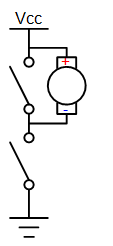
\includegraphics[width=0.33\columnwidth]{images-dis3/driver-half} \\ Half-bridge driver}
  \only<2>{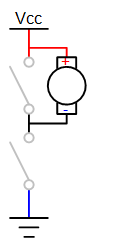
\includegraphics[width=0.33\columnwidth]{images-dis3/driver-half-off} \\ Motor off}
  \only<3>{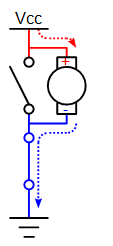
\includegraphics[width=0.33\columnwidth]{images-dis3/driver-half-on} \\ Motor on}
  \only<4>{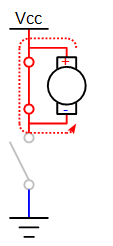
\includegraphics[width=0.33\columnwidth]{images-dis3/driver-half-brake} \\ Braking}
  \only<5>{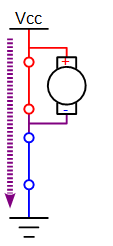
\includegraphics[width=0.33\columnwidth]{images-dis3/driver-half-shoot} \\ Shoot-through}
\end{figure}
\end{columns}
\end{frame}

\begin{frame}
\frametitle{H-Bridge Recap \small (for your reference)}
\begin{columns}[t]
\column{0.646\textwidth}
\begin{itemize}
  \item This driver design gives you forward, reverse, and braking using four transistors
  % TODO: explain name and rework diagrams in better format
  \item<2-> When all switches are off, no current can flow and the motor freewheels
  \item<3-> With an opposing pair of top and bottom switches on, current flows through the motor causing it to spin
  \item<4-> Turning on the opposite switches causes the motor to spin in the other direction
  \item<5-> Braking is accomplished by turning on both the top or both the bottom switches
\end{itemize}

\column{0.323\textwidth}
\begin{figure}
  \centering
  \only<1>{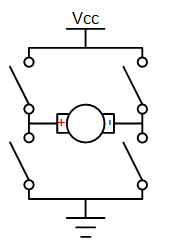
\includegraphics[width=0.33\columnwidth]{images-dis3/driver-h} \\ Half-bridge driver}
  \only<2>{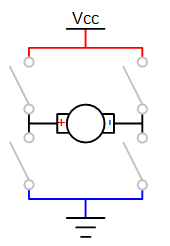
\includegraphics[width=0.33\columnwidth]{images-dis3/driver-h-off} \\ Motor off}
  \only<3>{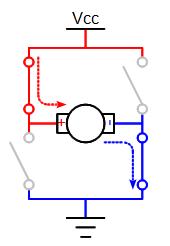
\includegraphics[width=0.33\columnwidth]{images-dis3/driver-h-fwd} \\ Forward}
  \only<4>{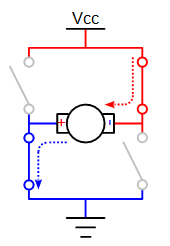
\includegraphics[width=0.33\columnwidth]{images-dis3/driver-h-rev} \\ Reverse}
  \only<5>{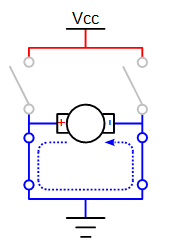
\includegraphics[width=0.33\columnwidth]{images-dis3/driver-h-brake} \\ Braking}
\end{figure}
\end{columns}
\end{frame}

%---------------------------------------------------------------------
\subsection{Humble Beginnings}

\begin{frame}
\frametitle{A Single Transistor MOSFET Motor Driver}
\begin{columns}[t]
\column{0.646\textwidth}
\begin{itemize}
  \item So I've got a demo circuit set up:
  \begin{itemize}
    \item All running off benchtop power supplies
    \item MOSFET switch on the low side (source to GND, drain to the motor)
    \item Function generator drives MOSFET gate
  \end{itemize}
  \item Basically, allows a logic-level signal (like from your microcontroller) to control a huge current source (to the motor)
  \begin{itemize}
    \item Note that most MCUs can only source / sink up to 25mA per pin
    \item But motors require many amps...
  \end{itemize}
\end{itemize}

\column{0.323\textwidth}
\begin{figure}
  \centering
  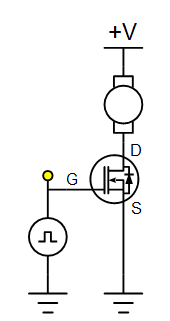
\includegraphics[scale=0.33]{images-dis3/driverckt-lowside} \\
  Motor Driver Circuit
\end{figure}
\end{columns}
\end{frame}

\begin{frame}
\frametitle{PWM Input Waveform}
\begin{columns}[t]
\column{0.646\textwidth}
\begin{itemize}
  \item Remember how PWM fades LEDs (checkpoint 1)?
  \begin{itemize}
    \item Same principle applies to motors
    \item Use highly efficient digital switches to approximate analog signal
  \end{itemize}
  \item Function generator creates a 1kHz PWM signal (square wave) at 20\% duty cycle
  \begin{itemize}
    \item When MOSFET is on, forward current goes through the motor, creating torque
    \item When MOSFET is off, no current through the motor, so just spins from inertia
  \end{itemize}
  \item Do this really fast and you control speed between ``full-on'' and ``full-stop''
\end{itemize}

\column{0.323\textwidth}
\begin{figure}
  \centering
  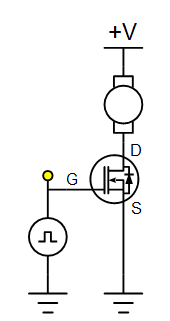
\includegraphics[scale=0.33]{images-dis3/driverckt-lowside} \\
  Motor Driver Circuit \\
  \hfill \\
  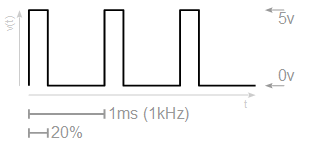
\includegraphics[width=1.0\columnwidth]{images-dis3/driverwave-demo} \\
  Gate Waveform
\end{figure}
\end{columns}
\end{frame}

\begin{frame}
\frametitle{Check your Understanding {\small (Live Demo Edition!)}}
\begin{columns}[t]
\column{0.646\textwidth}
\begin{itemize}
  \item I can adjust these PWM parameters: \\ frequency (period) and duty cycle
  \item What should I do to ...
  \begin{itemize}
    \item ... make the motor faster?
    \begin{itemize}
      \item<2-> Increase duty cycle (more time in accel)
    \end{itemize}
    \item ... make the motor slower?
    \begin{itemize}
      \item<3-> Decrease duty cycle (more friction time)
    \end{itemize}
  \end{itemize}
  \item What happens if ...
  \begin{itemize}
    \item ... I reduce the frequency?
    \begin{itemize}
      \item<4-> Motor chatter (significant accel and decel during each period)
    \end{itemize}
    \item ... I increase the frequency?
    \begin{itemize}
      \item<5-> Smoother operation, but thermal effects \\ (switching puts MOSFET through low-efficiency linear region) and slew
    \end{itemize}
  \end{itemize}
\end{itemize}

\column{0.323\textwidth}
\begin{figure}
  \centering
  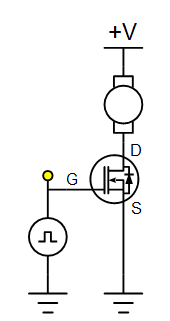
\includegraphics[scale=0.33]{images-dis3/driverckt-lowside} \\
  Motor Driver Circuit \\
  \hfill \\
  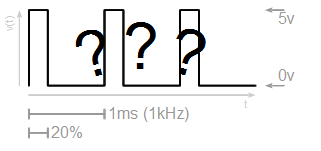
\includegraphics[width=1.0\columnwidth]{images-dis3/driverwave-questions} \\
  Gate Waveform
\end{figure}
\end{columns}
\end{frame}

%---------------------------------------------------------------------
\subsection{Velocity Sensing}

\begin{frame}
\frametitle{Sensing speed with back-EMF}
\begin{columns}[t]
\column{0.646\textwidth}
\begin{itemize}
  \item Recall: a spinning motor produces voltage
  \begin{itemize}
    \item ... which can be measured to sense speed!
  \end{itemize}
  \item The scope is connected to the motor leads
  \begin{itemize} % TODO: colorcode this
    \item Green probe on the positive motor lead (connected to the positive supply)
    \item Purple probe on the negative motor lead (connected to the MOSFET drain)
  \end{itemize}
  \item I want the voltage across the motor
  \begin{itemize}
    \item Use math mode (red) to get green - purple
  \end{itemize}
  \item<2-> ... now what about on a microcontroller?
  \begin{itemize}
    \item Sample both pins and subtract in software \\ (if sampling speed$\gg$motor time constant)
  \end{itemize}
\end{itemize}

\column{0.323\textwidth}
\begin{figure}
  \centering
  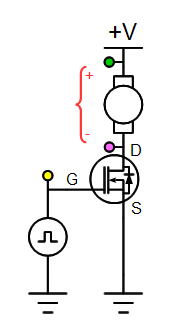
\includegraphics[scale=0.33]{images-dis3/driverckt-lowside-emf} \\
  Back-EMF measurement
\end{figure}
\end{columns}
\end{frame}

% TODO: add section on PMOS devices
%---------------------------------------------------------------------
\subsection{Gate Predriver} % [?? mins]

\begin{frame}
\frametitle{A High-Side Motor Driver}
\begin{columns}[t]
\column{0.646\textwidth}
\begin{itemize}
  \item Consider a MOSFET driving the high side
  \item What do you think would happen with the same drive waveform at the gate?
  \begin{itemize}
    \item<2-> Nothing! Insufficient gate voltage!
  \end{itemize}
  \item<2-> Remember: MOSFET on/off depends on voltage between \textbf{its} gate and source
  \begin{itemize}
    \item NOT referenced to the circuit ground
    \item But when on, source is at supply voltage
  \end{itemize}
  \item<2-> Must boost gate voltage above the supply
  \begin{itemize}
    \item Enter the gate predriver chip, MC33883
  \end{itemize}
\end{itemize}

\column{0.323\textwidth}
\begin{figure}
  \centering
  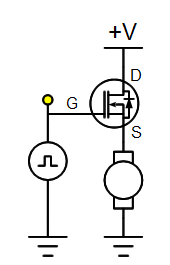
\includegraphics[scale=0.33]{images-dis3/driverckt-highside} \\
  High-side Driver
\end{figure}
\hfill \\
\pause
\begin{figure}
  \centering
  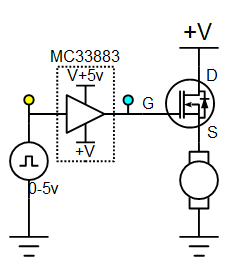
\includegraphics[scale=0.33]{images-dis3/driverckt-highside-boost} \\
  With Gate Boost
\end{figure}
\end{columns}
\end{frame}

\begin{frame}
\frametitle{MC33883 Gate Predriver}
\begin{columns}[t]
\column{0.646\textwidth}
\begin{itemize}
  \item Has four gate drivers:
  \begin{itemize}
    \item GATE\_HS\textit{x} pins, controlled by IN\_HS\textit{x}
    \begin{itemize}
      \item Boosts gate above Vcc when on, discharge to SRC\_\textit{x} when off
    \end{itemize}
    \item GATE\_LS\textit{x} output controlled by IN\_LS\textit{x} \\
    \begin{itemize}
      \item Translates to Vcc when on, discharge to GND when off
      \item Generate Vcc-level signals from 3.3v
    \end{itemize}
  \end{itemize}
  \item Designed to drive a H-bridge
  \begin{itemize}
    \item No shoot-through logic protection
    \item Can be used as 4 independent drivers
    \item Can use the GATE\_HS\textit{x} to apply higher gate voltage to low-side FETs
  \end{itemize}
\end{itemize}

\column{0.323\textwidth}
\begin{figure}
  \centering
  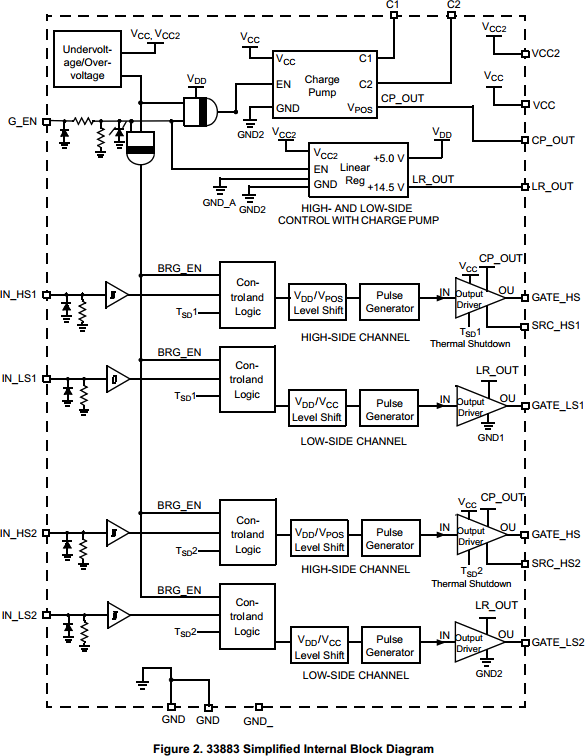
\includegraphics[width=1.0\columnwidth]{images-dis3/mc33883-blockdiagram} \\
  MC33883 \\ Functional Block \\
  {\tiny source: MC33883 datasheet, by Freescale}
\end{figure}
\end{columns}
\end{frame}

\begin{frame}
\frametitle{MC33883 Misc Tips \small (for your reference)}
\begin{columns}[t]
\column{0.646\textwidth}
Important specs from the datasheet
\begin{itemize}
  \item Minimum Vcc, Vcc2 of 5.5v
  \begin{itemize}
    \item and a maximum Vcc of 55v, Vcc2 of 28v
  \end{itemize}
  \item G\_EN pin as gate enable, set low to disable, set $>$4.5v to enable
  \begin{itemize}
    \item 3.3v logic-level drive will NOT work!
  \end{itemize}
  \item At Vcc=7.2v (maximum for Freescale Cup), charge pump output Vcp$\approx$12v
  \begin{itemize}
    \item Which is $\sim$4.5v over Vcc, sufficient to drive a high-side MOSFET
  \end{itemize}
  \item 3.3v logic comptible input ports
  \begin{itemize}
    \item Anything above 2.0v treated as high
    \item Anything below 0.8v treated as low
  \end{itemize}
  \item Maximum PWM frequency of 100kHz
\end{itemize}

\column{0.323\textwidth}
\begin{figure}
  \centering
  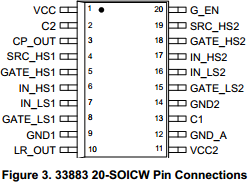
\includegraphics[width=1.0\columnwidth]{images-dis3/mc33883-pinning} \\
  {\small and the all-important} \\ Pinning Diagram \\
  {\tiny source: MC33883 datasheet, by Freescale}
\end{figure}
\end{columns}
\end{frame}

\begin{frame}
\frametitle{MC33883 Application Circuit \small (for your reference)}
\centering
Datasheet page 18 has all you need to know \\
\hfill \\
You can skip the Zener diodes and use independent MOSFETs, \\
but make sure to tie SRC\_\textit{x} to the MOSFET source of GATE\_HS\textit{x}
\begin{figure}
  \centering
  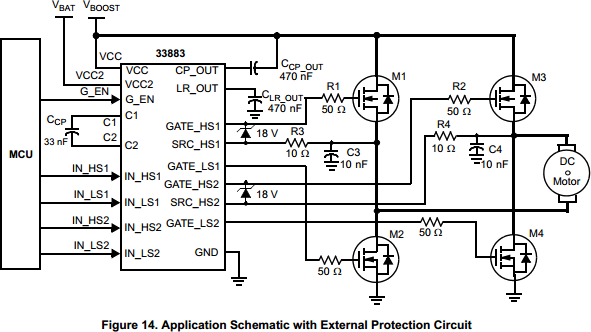
\includegraphics[width=0.5\columnwidth]{images-dis3/mc33883-application} \\
  MC33883 Application Circuit \\
  {\tiny source: MC33883 datasheet, by Freescale}
\end{figure}
\end{frame}

\begin{frame}
\frametitle{Charge Pump Theory \small (for your reference)}
\begin{columns}[t]
\column{0.646\textwidth}
So, how does the MC33883 generate gate voltages above Vcc?
\begin{itemize}
  \item Uses a switched-capacitor charge pump
\end{itemize} 
Let's start with a simple switched-capacitor voltage doubler circut...
\begin{itemize}
  \item Start by charging capacitor to Vcc
  \item<2-> Disconnect capacitor from supplies
  \begin{itemize}
    \item<2-> Capacitor retains its charge
  \end{itemize}
  \item<3-> Connect capacitor low-side to Vcc
  \begin{itemize}
    \item<3-> Capacitor high-side now at 2Vcc
  \end{itemize}  
  \item<4-> Connect capacitor to output filter
  \begin{itemize}
    \item<4-> Charge output filter to 2Vcc
  \end{itemize}  
\end{itemize}

\column{0.323\textwidth}
\begin{figure}
  \centering
  \only<1>{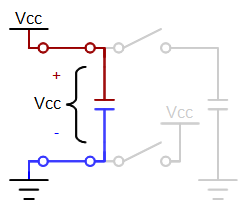
\includegraphics[width=1.0\columnwidth]{images-dis3/doubler-charge} \\ Capacitor charging}
  \only<2>{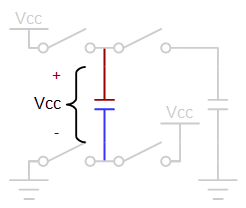
\includegraphics[width=1.0\columnwidth]{images-dis3/doubler-float} \\ Capacitor floating}
  \only<3>{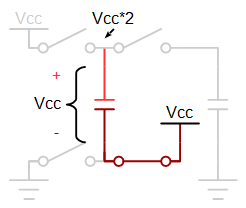
\includegraphics[width=1.0\columnwidth]{images-dis3/doubler-double} \\ Voltage doubled}
  \only<4>{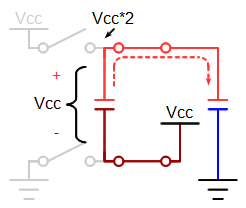
\includegraphics[width=1.0\columnwidth]{images-dis3/doubler-discharge} \\ Charge output}
\end{figure}
\end{columns}
\end{frame}

\begin{frame}
\frametitle{MC33883 Charge Pump \small (for your reference)}
\begin{columns}[t]
\column{0.646\textwidth}
MC33883's charge pump uses a oscillator and diodes instead of switches
\begin{itemize}
  \item When oscillator is low, capacitor is charged through diode
  \item <2-> When oscillator goes high, low-side of capacitor goes to Vcc
  \begin{itemize}
    \item <2-> High side of capacitor rises as well and charges CP through the diode
  \end{itemize}
  \item <2-> (this illustrates the concept but skips details like different voltages and diodes)
\end{itemize}

\column{0.323\textwidth}
\begin{figure}
  \centering
  \only<1>{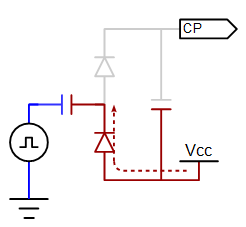
\includegraphics[width=1.0\columnwidth]{images-dis3/mc33883pump-charge} \\ Capacitor charging}
  \only<2>{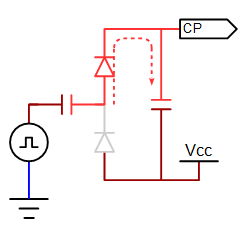
\includegraphics[width=1.0\columnwidth]{images-dis3/mc33883pump-discharge} \\ Charge output}
\end{figure}
\end{columns}
\end{frame}

\begin{frame}
\frametitle{Questions?}
\centering
{\huge got it?} \\
\vspace{20px}
\tiny{ready to pwn checkpoint 3?}
\end{frame}

%---------------------------------------------------------------------
\section{Wiring} % [?? mins]
%---------------------------------------------------------------------
\begin{frame}
\centering \huge Wiring
\end{frame}
%---------------------------------------------------------------------
\subsection{Basics}

\begin{frame}
\frametitle{Wire Types}
\begin{columns}[t]
\column{0.646\textwidth}
\begin{itemize}
  \item Solid
  \begin{itemize}
    \item A single solid chunk of copper conductor
    \item Rigid but inflexible: helpful in some cases
  \end{itemize}
  \item Stranded
  \begin{itemize}
    \item Made of individual strands of copper wire
    \item More flexible, especially when there are more (and thinner) strands
  \end{itemize}
  \item Wire gauge (size) is by cross-section area
  \begin{itemize}
    \item So stranded wire has ``thicker'' conductor, because of space between strands
  \end{itemize}
  \item Which is more resistant to breaking from flexing? Why?
  \begin{itemize}
    \item<2-> Stranded wire: more flexible %% TODO: WHAT IS THE MECH THEORY BEHIND THIS?
  \end{itemize}
\end{itemize}

\column{0.323\textwidth}
\begin{figure}
  \centering
  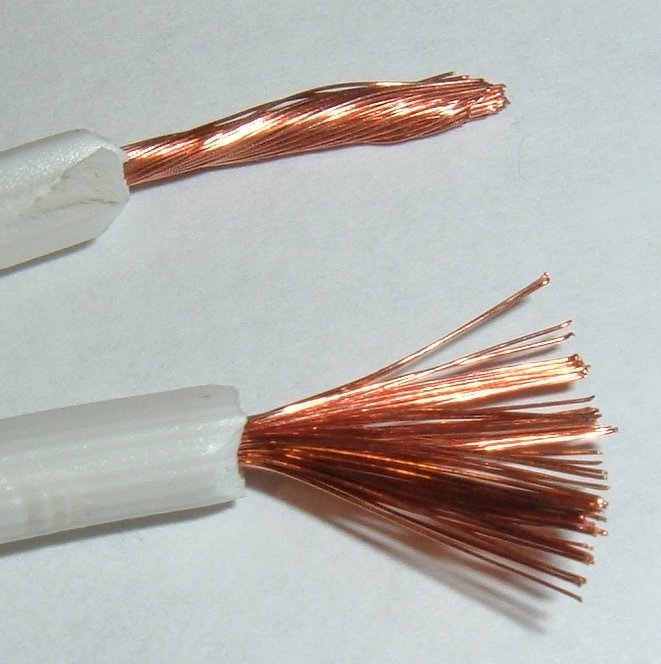
\includegraphics[width=1.0\columnwidth]{images-dis3/stranded_lamp_wire} \\
  Stranded Wire \\
  {\tiny source: Wikipedia, Scott Ehardt}
\end{figure}
\end{columns}
\end{frame}

%---------------------------------------------------------------------
\subsection{Connectors}

\begin{frame}
\frametitle{Anderson Powerpole}
\begin{columns}[t]
\column{0.646\textwidth}
\begin{itemize}
  \item Physically and electrically hermaphroditic
  \begin{itemize}
    \item Physically can't insert it the wrong way
    \item Both sides of the connector are identical
  \end{itemize}
  \item We're standardizing on the PP15/30/45
  \begin{itemize}
    \item We have many 15-amp contacts, suitable for 16-20 AWG wire
    \item 30-amp contacts also available for larger (12-14 AWG) wire
  \end{itemize}
  \item Complete set of tools available
  \begin{itemize}
    \item Crimper and insertion tool
  \end{itemize}
  \item Use this for all your high-power connectors
  \begin{itemize}
    \item Battery to board, driver to motor, ...
  \end{itemize}
  \item Quick demo
\end{itemize}

\column{0.323\textwidth}
\begin{figure}
  \centering
  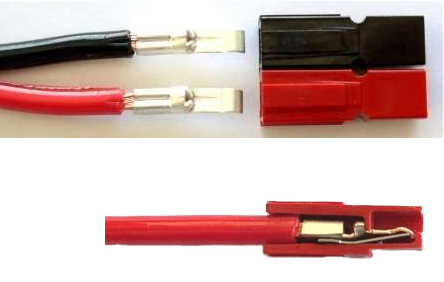
\includegraphics[width=1.0\columnwidth]{images-dis3/powerpole_cutaway} \\
  Powerpole Connector \\
  {\tiny source: Wikipedia, Cqdx}
\end{figure}
\end{columns}
\end{frame}

% TODO: Add IDC crimps

\begin{frame}
\frametitle{Questions?}
\centering
{\huge makes sense?} \\
\vspace{20px}
\tiny{tl;dr: use stranded wire}
\end{frame}

%---------------------------------------------------------------------
\section{Servomotors} % [?? mins]
%---------------------------------------------------------------------
\begin{frame}
\centering \huge Servomotors
\end{frame}
%---------------------------------------------------------------------
\subsection{Intro}

\begin{frame}
\frametitle{Intro}
\begin{columns}[t]
\column{0.646\textwidth}
\begin{itemize}
  \item Servomechanism: device using feedback loop to provide control
  \item RC cars use servomotor-actuated steering
  \begin{itemize}
    \item Motor senses output shaft position and adjusts to hit commanded angle
    \item Freescale Cup allows the Futaba S3010
  \end{itemize}
  \item 3-wire standard servo cable:
  \begin{itemize}
    \item white / yellow / orange: signal
    \item red: positive supply voltage
    \item black / brown: negative supply voltage
  \end{itemize}
\end{itemize}

\column{0.323\textwidth}
\begin{figure}
  \centering
  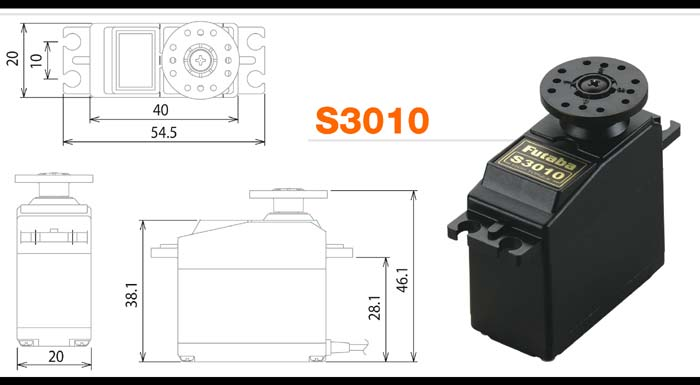
\includegraphics[width=1.0\columnwidth]{images-dis3/specs-futm0043} \\
  S3010 Servomotor \\
  {\tiny source: Futaba, www.futaba-rc.com}
\end{figure}
\end{columns}
\end{frame}

\begin{frame}
\frametitle{Inside a Servo {\small (for your reference)}}
will be on the discussion slides posted to the site
\end{frame}

%---------------------------------------------------------------------
\subsection{Protocol}

\begin{frame}
\frametitle{PWM Control}
\begin{columns}[t]
\column{0.646\textwidth}
\begin{itemize}
  \item NOT the same PWM as motor control
  \item Servo setpoint by width of high pulse
  \begin{itemize}
    \item Allowable width between 1ms - 2ms
    \item 1.5ms to set setpoint to center
  \end{itemize}
  \item Servo expects regular pulses
  \begin{itemize}
    \item Wikipedia says at least once per 20ms
    \item But varies from model to model
    \item Servo will timeout (and turn off) if it doesn't get regular data
  \end{itemize}
\end{itemize}

\column{0.323\textwidth}
\begin{figure}
  \centering
  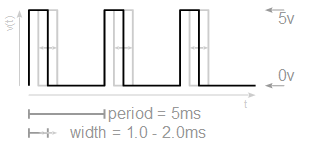
\includegraphics[width=1.0\columnwidth]{images-dis3/pwmwave-multi} \\
  PWM Waveform
  % TODO: TO SCALE
\end{figure}
\end{columns}
\end{frame}

\begin{frame}
\frametitle{Check your Understanding {\small (Live Demo Edition!)}}
\begin{columns}[t]
\column{0.646\textwidth}
\begin{itemize}
  \item So I have a function generator PWM set at Vpp=5v, Vdc=2.5v, f=200 Hz, 30\% duty
  \item What is the period and pulse width?
  \begin{itemize}
    \item<2-> period=5ms, pulse width=1.5ms
  \end{itemize}
  \item What will the setpoint be?
  \begin{itemize}
    \item<3-> Dead center
  \end{itemize}
  \item What do I do to move it to one side?
  \begin{itemize}
    \item<4-> Adjust the duty cycle, say, downwards
  \end{itemize}
  \item Now I want to move it hard other side. What do I set the width and duty cycle?
  \begin{itemize}
    \item<5-> pulse width=2.0ms, duty cycle=40\%
    \item<5-> Beware of mechanical blockage stalling!
  \end{itemize}
\end{itemize}

\column{0.323\textwidth}
\begin{figure}
  \centering
  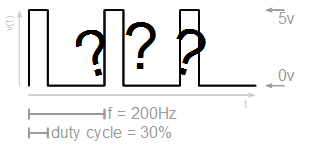
\includegraphics[width=1.0\columnwidth]{images-dis3/pwmwave-questions} \\
  PWM Waveform
\end{figure}
\end{columns}
\end{frame}

\begin{frame}
\frametitle{Questions?}
\centering
{\huge got this down?} \\
\vspace{20px}
\tiny{we all know how to steer now, right?}
\end{frame}

%---------------------------------------------------------------------
\section{Summary} % [?? mins]

\begin{frame}
\frametitle{Summary}
Summary
\begin{itemize}
  \item Apply PWM waveform to motor driver circuits to control speed
  \item Use a gate predriver to drive MOSFETs from wimpy 3.3v logic
  \item Steering servos controlled with a different kind of PWM
  \item Use stranded wire
\end{itemize}
Parts Handout
\begin{itemize}
  \item Get 3 NDP7060 MOSFETs per team
  \item Re-use your LED perfboards for the motor driver checkpoint
  \item SOIC carriers and MC33883 chips to be handed out Friday
  \item Need help soldering SOIC? Come to office hours!
\end{itemize}
\end{frame}

\end{document}
